%all packages here
\documentclass[]{article}
%\documentclass[journal]{IEEEtran}
%\usepackage{url}
\usepackage{lettrine}
\usepackage{amsmath}
\usepackage{amssymb}
\usepackage{graphicx}
\usepackage{cite}
\usepackage{float}
\begin{document}
\title{Playing with \LaTeX{}}
\author{Ananya}
%\date{June 41 2020}
\maketitle

\begin{abstract}
This is the abstract.
\end{abstract}
This is the body.\cite{wikilatex}
\section{Reptiles}
Reptiles are tetrapod animals in the class
\emph{Reptilia}, \textbf{comprising} today's turtles, crocodilians, snakes, amphisbaenians, lizards, tuatara, and their extinct relatives. 
\subsection{Snakes}
Snakes are elongated, \textbf{legless}, carnivorous reptiles of the suborder \emph{Serpentes}. 
\subsubsection{Cobra}
Cobra is the common name of various elapid snakes, most of which belonging to the genus \emph{Naja}. 

\section{Exercise : Text Manipulation}
\lettrine{S}{carlett} O'Hara was not beautiful, but men seldom realized it when caught by her charm as the Tarleton twins were. In her face were too sharply blended the delicate features of her mother, \textit{a Coast aristocrat of \emph{French} descent, and the heavy ones of her florid \emph{Irish} father}. But it was an arresting face, pointed of chin, square of jaw. \underline{Her eyes were pale green without a touch of hazel}, starred with bristly black lashes and slightly tilted at the ends. Above them, her \textbf{\textit{thick black brows}} slanted upward, cutting a startling oblique line in her magnolia-white skin - that skin so prized \\by Southern women and so carefully guarded with bonnets, veils and mittens against hot Georgia suns.
\par Seated with Stuart and Brent Tarleton in the cool shade of the porch of Tara, her father's plantation, that bright April afternoon of 1861, she made a pretty picture. 


\section{Equations and Symbols}
\subsection{Math Mode}
Square roots may be positive or negative. For example, $\sqrt{9} = \pm 3$.\\ $\sqrt{4}$
Here's a chemical equation: $Na_2CO_3 + H_2SO_4 = Na_2SO_4 + H_2O + CO_2 $
\subsection{Equation}

Fermat's Last Theorem  states that no three positive integers $a$, $b$, and $c$ satisfy the equation \ref{fermat_eq} \cite{wiki:fermat}. 
\begin{equation}
\label{fermat_eq}
a^n + b^n = c^n \qquad n \in \mathbb{Z}, \ n>2
\end{equation}
Using align:
\begin{align}
4x + 5 & = 13 \\
4x &= 13-5\\
4x &= 8\\
x &= 8/4\\
x&=2
\end{align}
The following equations hold for ideal gases.
\begin{subequations}
\begin{align}
\intertext{Boyle's law:}
P&=\frac{k}{V} \\ 
\intertext{Charles' law:}
V&=kT\\
\intertext{Ideal Gas law}
PV&=nRT
\\
a &= b
\end{align}
\end{subequations}
More random equations:
\begin{align}
&\sum_i x^P_{i,j} = 1 \forall j \\
&w^{mon} \in \{0,1\}  \\
&\frac{1}{2} y_{j} \geq 1 \\
&r_{j} = 10\% 
\end{align}
Random text 1.
\begin{table}[H]

\begin{center}
\begin{tabular}{c|c|c}
\textbf{Starting Letter}&\textbf{Word} &\textit{another word}\\
A&apple& avocado \\
B&ball & breeze\\
C&cat & chef
\end{tabular}
\end{center}
\caption{Table of Words}
\label{tab1}
\end{table}
Random text 2.

\begin{figure}[h]
\begin{center}
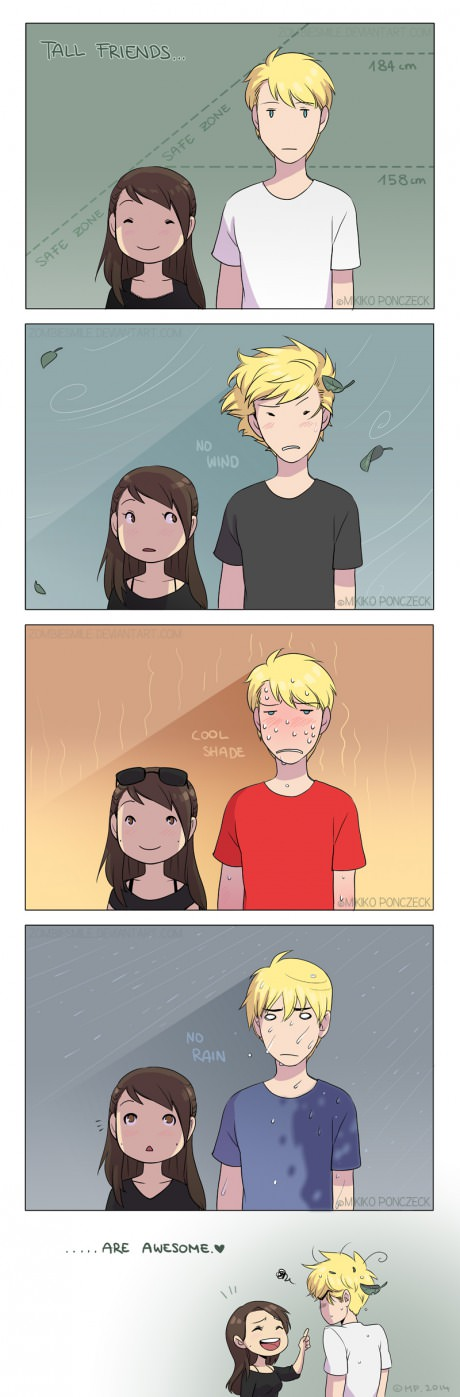
\includegraphics[width=70mm,height=70mm]{tall_fr.jpg} 
\caption{{\bf Tall Friends are Awesome!}}
\label{fig1}
\end{center}

%\end{center}
\end{figure}

\section{My Textbooks:}
\begin{itemize}
\item B.V. Ramana - Higher Engineering Mathematics
\begin{enumerate}
    \item object 1
    \item object 3
\end{enumerate}
\item Richard Feynman -  Lectures on Physics
\item Boylested and Nashelsky - Basic Electronics \cite{bohra}
\end{itemize}

\section{My Textbooks:}
\begin{enumerate}
\item B.V. Ramana - Higher Engineering Mathematics
\item R. Feynman Lectures on Physics
\item Boylested and Nashelsky- Basic Electronics
\item ImageNet %\cite{imagenet}
\end{enumerate}

\bibliographystyle{IEEEtran}
\bibliography{bibmil}
\end{document}

